\documentclass[12pt,onecolumn]{IEEEtran}
\usepackage{amsmath ,amssymb,euscript ,yfonts,psfrag,latexsym,dsfont,graphicx,bbm,color,amstext,wasysym,subfig,flushend,parskip}
\usepackage{bm,cite,soul,url}
\usepackage{verbatim}
\usepackage[normalem]{ulem}
\usepackage{amsthm}
%\usepackage{refcheck}
%\usepackage{showkeys}
%\usepackage{epstopdf,hyperref,pdfsync,url}
\graphicspath{{./},{./figures/}}
\newcommand{\mR}{{\mathbb R}}
\newcommand{\D}{{\mathbb D}}
\newcommand{\E}{{\mathbb E}}
\newcommand{\mcN}{{\mathcal N}}
\newcommand{\mcR}{{\mathcal R}}
\newcommand{\diag}{\operatorname{diag}}
\newcommand{\tr}{\operatorname{trace}}
\newcommand{\ignore}[1]{}
\newcommand{\mike}{\color{magenta}}

\newcommand{\blue}{\color{blue}}
\newcommand{\red}{\textcolor{red}}

\newcommand{\bQ}{{\bm{Q}}}
\newcommand{\bPi}{\bm{\Pi}}
\newcommand{\bv}{{\bm{v}}}
\newcommand{\balpha}{{\bm{\alpha}}}
\newcommand{\bbeta}{{\bm{\beta}}}
\newcommand{\bq}{{\bm{q}}}
\newcommand{\bp}{{\bm{p}}}
\newcommand{\bbf}{{\bm{f}}}
\newcommand{\differential}{{\mathrm{d}}}

\newtheorem{claim}{Claim}

\def\spacingset#1{\def\baselinestretch{#1}\small\normalsize}
\setlength{\parskip}{10pt}
\setlength{\parindent}{20pt}
\spacingset{1}

\definecolor{grey}{rgb}{0.6,0.6,0.6}
\definecolor{lg}{rgb}{0.6,.6,0.6}
\newcommand{\nib}{\noindent  {\bf Response:} }

\begin{document}
%\newcommand{\bp}{{\bm{p}}}
\noindent
{\large {\bf Revision of
Manuscript Number}: IEEE-TPWRS-01391-2021, version 1\hfill \today\\[.1in]
{\bf Journal}: IEEE Transactions on Power Systems \\[.1in]
{\bf Author}: Abhishek Halder, Kenneth F. Caluya, Pegah Ojaghi, Xinbo Geng}\\



\section*{\large \bf Response to decision:}

{\noindent\blue
The perceptive input from all reviewers and the AE are much appreciated. 

Please find below itemized responses to the individual comments addressing the concerns and detailing the revisions. All the edits in the revised manuscript are marked in blue.\\

\noindent
Sincerely,\\
The authors
}


%%%%%%%%%%%%%%%%%%%%%%%%%%%%%%%%%%%%%%%%%%%%%%%%%%%%%%%%%%%%%%%%%%%%%%%%%%%%%%%%%%%%%%%%%%%%

%\newpage
\spacingset{1}

\section*{\large \bf Response to AE:}

\noindent
{\bf AE.1. Comments by AE}:\\
{\em The authors are requested to revise and resubmit their paper after addressing reviewer feedback. Of particular importance is that reviewers point out the model leveraged for analysis is overly simplistic.}

{\nib {\blue We are indebted to the AE and the reviewers for their help to improve the manuscript.

In addition to the itemized responses to the reviewers' comments and the corresponding revisions marked in blue in the manuscript, we have made the \ul{following additional fixes and improvements} (also marked in blue in the revised manuscript):\\
(i) In equation (8), we corrected a typo in its right hand side: the second summand runs over pairs $(i,j)$ such that $i<j$.\\
(ii) To make the presentation tighter, the Appendix appearing in the previous version has been eschewed. We have accordingly adjusted and condensed the material in Sec. III-D of the revised manuscript.\\
(iii) Some mathematical typos have been fixed in the revised manuscript's Sec. III-C and III-D.

{\red{Regarding the usage of simple model, please see our response to comment \textbf{R3.1} and \textbf{1.3, sub-comment (1)}. In summary, the current state-of-the-art in power system literature for this problem is ref. [45] with second order dynamics + single machine infinite bus ($n=1$ in our manuscript's notation). Given this context, our manuscript enables a new kind of computation that can handle moderately large $n$ with second order sample path dynamics. This computation is online and approximates neither the statistics nor the dynamics.  \ul{We clarify two important points here}:\\(i) The proposed proximal recursion framework on the space of probability measures is not conceptually limited by the second order dynamics, and we expect follow up research to design custom proximal recursions for higher order synchronous machine models. In this sense, the present paper should be seen as the stepping stone laying the foundation for handling more complex dynamical models. The authors have been completely up front by explicitly mentioning this in the Conclusions section. We have also reiterated the same in this rebuttal.\\(ii) Deriving proximal recursion requires understanding the generalized gradient flow structure over probability measures. Our research disposition is that one cannot bypass understanding the generalized gradient flow structure for the simpler second order sample path dynamics before attempting the same for more complex sample path models. In fact, a significant contribution of our article, in the authors' opinion, is that it distills out what exactly is mathematically challenging.}} 
}}


\noindent
{\bf AE.2. Comments by AE}:\\
{\em Authors are also encouraged to revisit their overview of prior art.}

{\nib {\blue Following the suggestions, the revised manuscript has expanded the overview of prior art. Specifically, we have included \ul{two new references [22], [23] on stochastic differential algebraic equations (SDAEs) and cited them inline in Sec. I.1, second paragraph, as detailed in our response to the comment \textbf{R3.2} in this document}. This includes the reference suggested in comment \textbf{R1.3}. \ul{We have also included the reference suggested in comment \textbf{R4.4}; this is reference [28] in the revised manuscript. Its inline citation is in Sec. I.1, last paragraph, first sentence}.}}


\noindent
{\bf AE.3. Comments by AE}:\\
{\em Presentation of technical points and results can also be improved.}

{\nib {\blue We have made several updates to clarify the technical issues and to improve the presentation.

\ul{Following the comment \textbf{R4.3} to improve the presentation, in the revised manuscript, we have expanded the last two paragraphs of Sec. III-A with a new reference [50]}. Please see our response to that comment below for details. 

\ul{As detailed in the response to comment \textbf{R3.4}, in the revised manuscript, we have enlarged Figures 5 and 6, and expanded the plot in Fig. 6}. There we also explained why those plot styles are used.

\ul{Furthermore, Fig. 7 in the revised manuscript has also been expanded to include the univariate angular velocity transient marginal plots for all the five generators of the IEEE 14 bus system; previous version had this plot only for the generator 4 (buss 6)}.

{\red{New plots}}
}}




%%%%%%%%%%%%%%%%%%%%%%%%%%%%%%%%%%%%%%%%%%%%%%%%%%%%%%%%%%%%%%%%%%%%%%%%%%%%%%%%%%%%%%%%%%%%

\newpage
\spacingset{1}

\section*{\large \bf Response to Reviewer \#1:}


\noindent
{\bf R1.1. Comment by reviewer}:\\
{\em The original contribution of the article is not clear.  Indeed, what is original new from this article, not the summary from existing techniques?}


{\nib {\blue The original contribution of this article is to design an algorithm for \emph{online nonparametric} computation of the joint state PDFs subject to stochastic uncertainties (initial conditions, parameters, process noise and combinations thereof) in power system dynamics. 

The qualifier ``online" means that it is not a variant of Monte Carlo where samples are first propagated \ul{and then} a function approximation is performed offline to estimate the joint state PDF at a snapshot. The qualifier ``nonparametric" means that neither the statistics nor the dynamics are approximated \emph{a priori}. This is novel because the existing power systems literature makes at least one of the aforesaid approximations. The state-of-the-art in power system literature is discussed in Sec I.1. More importantly, Sec. I.2 details why the state-of-the-art is what it is. \ul{We specifically explain the contribution of this article in Sec. I.3 titled ``Contributions of this paper".}
}}



\noindent
{\bf R1.2. Comments by reviewer}:\\
{\em The structure of the article should be highly improved. A large portion of the contexts is simply repeating the well-known power system classical model, kroon reduction, and the FPF equations.  Only from section IV, page 6, I can see some of the proposed weighted points methods.}


{\nib{ \blue We thank the reviewer for this comment. This paper is \emph{not} about novel implementation of an existing idea. The idea itself is new and consequently needs to be contextualized and developed in the paper. \ul{The discussion toward the end of Sec. II and that in Sec III are, in our opinion, more fundamental contribution than the implementation in Sec. IV. Those parts of the paper really mark the innovation since they explain why someone, even if conversant in infinite dimensional gradient flow literature, cannot directly apply existing techniques to this problem. Then Sec. III-C and III-D explain how to circumvent the specific difficulties arising in this problem. A reader jumping to Sec. IV assuming that everything before that is known, would be completely mistaken}. Notice that we clearly laid out the structure of this paper (which section does what) in the paragraph right before Sec. II starts.}}


\noindent
{\bf R1.3. Comments by reviewer}:\\
{\em I have major doubts about the model used in the article for the following reasons.\\
(1)     The paper claim the proposed method can propagate stochastic uncertainties in realistic power networks. However, only a classical model is used, which is not realistic at all.\\
(2)     Why do active power and reactive power from load have no randomness at all. This is too unrealistic.\\
(3)     The diffusion term of this article is only considered in the frequency. The process noise in the rotor angle is fully ignored. This is also unreasonable.\\
To improve your work, I highly suggested the authors follow [R1], which is missing in your literature but can help the authors better know Power system SDE.  Also, it is suggested to introduce the OU process to model the randomness in the load, which cannot be ignored in practice.\\
R1. A systematic method to model power systems as stochastic differential-algebraic equations, F. Milano, R. Zarate-Minano, IEEE Transactions on Power Systems, 28(4), 4537-4544.}

{\nib{ \blue \ul{Our responses to the sub-comments below}.

(1) \textbf{Regarding usage of classical model:} Whether a model is relevant depends on the problem context. As pointed out in the last paragraph of Sec. II-B, the current state-of-the-art in power system literature for the problem we are addressing is ref. [45] with second order dynamics + single machine infinite bus ($n=1$ in our manuscript's notation). Given this context, our manuscript enables a new kind of computation that can handle moderately large $n$ with second order sample path dynamics. This computation is online and approximates neither the statistics nor the dynamics.  \ul{We clarify two important points here}:\\ \textbf{[1a]} The proposed proximal recursion framework on the space of probability measures is not conceptually limited by the second order dynamics, and we expect follow up research to design custom proximal recursions for \ul{higher order synchronous machine models}. In this sense, the present paper should be seen as the stepping stone laying the foundation for handling more complex dynamical models. \ul{The authors have been completely up front by explicitly mentioning this in the Conclusions section}. \\ \textbf{[1b]} Deriving proximal recursion requires understanding the generalized gradient flow structure over probability measures. \ul{Our research disposition is that one cannot bypass understanding the generalized gradient flow structure for the simpler second order sample path dynamics before attempting the same for more complex sample path models}. In fact, a significant contribution of our article, in the authors' opinion, is that it distills out what exactly is technically challenging and what are the peripheral issues.

(2) \textbf{Regarding randomness in active and reactive power:} {\red{TBD}} 

(3) \textbf{Regarding the diffusion term:} The reason why the diffusion term is present in the RHS of (1b) but not in the RHS of (1a) is because (1) is the state space representation of the second order Langevin dynamics (6). For the Langevin dynamics (6), its corresponding It\^{o} SDE \ul{has to be} (1). This is simply re-writing of a second order differential equation as an equivalent system of first order differential equations. There is no extra assumption here. \ul{Indeed, it is mathematically incorrect to add a noise term in the RHS of (1a) while claiming consistency with (6)}.

\ul{Notice that the absence of additive noise in the RHS of (1a) does \emph{not} imply that the rotor angles are deterministic trajectories}. The reason why the rotor angles are stochastic processes is because the process noise in (1b) affects the rotor angle sample paths via dynamical nonlinear coupling with the angular velocities, i.e., these are second order stochastic effects. \ul{In short, the noise in rotor angles is \emph{not} ignored; in fact the rotor angles are nonlinearly colored (i.e., non-white) noisy sample paths}. 

This reviewer may also have misunderstood in thinking that a model that has additive noise in the RHS of \emph{all} SDE components is somehow more general than the case where the additive noise terms are absent from some but not all components of an SDE RHS. \ul{In reality, the complexity is in the other way around}. The SDEs of the form (1) are the so-called ``degenerate It\^{o} SDEs" which are much more difficult to analyze than the non-degenerate versions (noise in the RHS of all SDE components). For instance, this degeneracy makes the joint PDF evolution equation (10) a \emph{kinetic} Fokker-Planck PDE, which is different in structure than the standard Fokker-Planck a.k.a. Kolmogorov's forward PDE. \ul{The gradient flow structure and the associated measure-valued proximal recursions for the kinetic Fokker-Planck PDE are less understood than the same for the standard Fokker-Planck PDE. This is exactly why the methodological contribution of this paper is important, even if one completely ignores the algorithmic contribution}. 

\textbf{Regarding the reference [R1]:} \ul{In the revised manuscript, we have included the ref. [R1] suggested by the reviewer with inline citation in Sec. I.1, toward the end of second paragraph. Please note that the topic of [R1] is different from the topic of our paper. We are interested in how to perform online nonparametric computation of transient joint state PDFs}. Our computation is different from Monte Carlo.

\textbf{Regarding OU process in load:} \ul{The reviewer might have missed the following key point of our paper}. The Kron reduced second order stochastic model implies that in the unreduced sense, the load dynamics was first order noisy Kuramoto, in addition to the synchronous machine dynamics being second order noisy Kuramoto. Therefore, we do have stochastic load dynamics, which is in fact more realistic than OU process model. While OU process assumes linear drift with constant diffusion, whereas our setting considers the load SDEs having drifts with trigonometric nonlinearity and constant diffusion.

}}



\noindent
{\bf R1.4. Comments by reviewer}:\\
{\em There is no comparison of the proposed method compared with other state-of-the-art methods. Therefore, it is hard for the readers to judge the importance of this article.}

{\nib{ \blue {\red{TBD}}.}}


\noindent
{\bf R1.5. Comments by reviewer}:\\
{\em Contributions are over-claimed in this article:\\
(1) The scalability of the proposed method cannot convince the readers since you are using a too simple model and ignored many important random dimensions from the loads.\\
(2) The proposed method claims to be nonparametric, however, all the inputs are assumed to be either wiener process or uniform distribution, which are all parametric distributions.\\
(3) If the ``nonparametric" is only referred to the output PDF, I would not think of it as a major contribution since there are a lot of existing techniques that can depict nonparametric PDF.}

{\nib{ \blue \ul{Our responses to the sub-comments below}.

(1) \textbf{Regarding simple model and ignoring the randomness in loads}: Please refer to our response to \textbf{R1.3, sub-comment (1)} where we explained why this model is relevant for this particular problem, and why this is not limiting to our methodological contribution. In response to \textbf{R1.3, last unnumbered sub-comment in bold text: ``Regarding OU process in load"}, we explained that we are not ignoring randomness from loads.

(2) \textbf{Regarding nonparametric}: \ul{We are \emph{not} making any parametric assumptions}. Our usage of the word ``nonparametric" is standard as in mathematical statistics literature. That the additive noise process is Wiener does not invite any loss of generality since if it was colored, we could always re-cast the same in our SDE form via a linear map. \ul{Furthermore, we have zero assumptions on the initial joint state PDF $\rho_{0}$ and on the joint PDF of the parameters appearing in the model. As a matter of fact, we don't even need to know the functional form of these joint PDFs. For instance, our framework remains unchanged if we are given the initial joint state and parameter distributional data as numerical table containing samples from these joints \emph{as well as} the joint PDF values evaluated at those samples}. The latter might be coming from some measurement-based sensor fusion/Bayesian algorithm. The specific product von Mises and uniform PDFs in Sec. V-A and V-B are only used for generating example data to perform our illustrative numerical simulations. \ul{This again underscores how looking into numerical simulations without contemplative reading and understanding of the earlier Sections may lead to misleading conclusions}.

(3) \textbf{Regarding depict nonparametric PDF}: \ul{This paper is not about nonparametric \emph{depiction} but about nonparametric \emph{computation} of the transient joint state PDFs}. For example, Monte Carlo followed by function approximation via Kernel density estimates and its variants, or other function approximants (e.g., RBF, Gaussian mixture, neural networks) are all parametric methods. We enable computing the value of joint state PDF at a time-varying sample location \emph{online (not as offline post-processing)} without assuming any functional representation of the transient joint which the computed values correspond to. Notice that we are doing this joint computation without gridding the state space, which would be impossible had we followed the traditional scientific computing route: finite element/volume methods, tensor decomposition techniques etc. \ul{We believe the proposed computational framework is novel, highly non-trivial and is specifically useful in this power system uncertainty propagation context}.
}}


\noindent
{\bf R1.6. Comments by reviewer}:\\
{\em The simulation time is too short to convince the readers. Only 1 second is considered here. Note that the errors can be quickly accumulated in the iteration.}

{\nib{ \blue {\red{TBD.}}}}


\noindent
{\bf R1.7. Comments by reviewer}:\\
{\em It is suggested to count the total computing time, not on each step.}

{\nib{ \blue While the depiction of the per-step computational times in Figs. 8 and 9 in the revised manuscript are somewhat unconventional, we explain why we choose to plot that way. \ul{To aid clarity, in the revised manuscript, we have added an excerpt of the following at the end of Sec. V-A.}

At each fixed physical time $t_{k}=kh$, $k\in\mathbb{N}$, where $h$ is the fixed step-size, we perform the proximal update $\varrho_{k-1}\mapsto\varrho_{k}$ via Algorithm 1. This proximal update has no analytical solution and instead requires execution of a contractive fixed point recursion. The physical time $t_{k}$ is ``frozen" (zero-order-hold) during the fixed point recursions underlying this one-step proximal update. \ul{To claim that the proposed method is practical, we therefore, need to demonstrate that the computational timescale is faster than the physical timescale, i.e., computational times needed to complete the zero-order-hold fixed point recursions are orders-of-magnitude faster than $h$, the step-size of physical time}. On the other hand, theoretical consistency (see the unnumbered equation after (26), before Sec. IV) requires that $h$ itself should be small. Thus, even if one has a provably convergent algorithm that can perform the one step proximal update, it is not clear \emph{a priori} if the computational time needed to do so can be much faster than $h$. If not, then the method would be statistically consistent but practically not useful. The Figs. 8 and 9 in the revised manuscript show that the computational time needed to perform the proximal updates, for all $t_{k}$, are indeed orders-of-magnitude faster than $h$.}}


\noindent
{\bf R1.8. Comments by reviewer}:\\
{\em If the proposed method depends on the Kronecker product, how can it be scaled to a higher dimension?}

{\nib{ \blue The proposed method \ul{does not entail computation of a Kronecker product}. In the manuscript, the Kronecker product with the $2\times 2$ identity matrix appeared in the definition of the change-of-variable (17). \ul{Its only purpose is to define} that change-of-variable, and \ul{thereby derive} the PDE in the new variables. The proximal recursion (for the PDE thus derived) detailed in Algorithm 1 \ul{does not have any Kronecker product computation}.}}


\noindent
{\bf R1.9. Comments by reviewer}:\\
{\em beta is undefined in equation (15a).}

{\nib{ \blue Thanks for the comment. The $\beta$ in (15a) is the same $\beta$ in (16), as in part of the same sentence. \ul{To avoid any confusion, in the revised manuscript, we have moved the phrase ``for some $\beta>0$" in (15a)}.}}



%%%%%%%%%%%%%%%%%%%%%%%%%%%%%%%%%%%%%%%%%%%%%%%%%%%%%%%%%%%%%%%%%%%%%%%%%%%%%%%%%%%%%%%%%%%%


\newpage
\section*{\large \bf Response to Reviewer \#2:}

\noindent
{\bf R2.1. Comments by reviewer}:\\
{\em Overall, the paper is well-written and theoretically sound.}

{\nib \blue{Thank you for the kind and encouraging remarks.}}


\noindent
{\bf R2.2. Comments by reviewer}:\\
{\em The paper's language and presentation make it seem like it is more oriented towards the applied mathematics and control communities. It is highly suggested that the authors revise the exposition of ideas and concepts, putting more emphasis on the power system so that it can be well-understood by the power system experts.}

{\nib \blue{We appreciate the comment. \ul{In the revised manuscript, we have made some changes toward this direction. This includes slightly expanded overview of the related power system literature (see the two sentences added in Sec. I.1, second paragraph with two new references [22], [23]), citing recent reference [28] in Sec. I.1, third paragraph. Please note that the literature review in Sec. I.1 is completely based on the power system literature}.

Having said that, we believe our technical contribution is indeed interdisciplinary in the sense it is not mere translational research. In other words, we are not simply importing ideas from a different domain and applying them to a power system problem. Instead, we make novel contributions at the (possibly unanticipated) intersection of two areas: measure-valued gradient flows and power system dynamics. The presentation of the paper reflects the same, perhaps rightfully so. Notice in particular that our presentation is bottom-up: we start from power system literature review and mention that the problem addressed in our paper was already recognized as a technical challenge in that literature. We move onto the theoretical ideas and tools much later in the manuscript, as the build up demands.

We expect a significant share of the readers of this work to be power system engineers, but not exclusively so since this contribution will also be of interest to the researchers in control, optimization and applied mathematics. We do not believe this issue is exceptional for our paper since several high impact papers in the IEEE Trans. Power Systems were indeed at the intersection of these areas, and are not only well-read by the researchers from either side but these works have positively contributed toward increasing interdisciplinary research collaboration.}}


\noindent
{\bf R2.3. Comments by reviewer}:\\
{\em How will the proposed approach be used for the cases in which dependencies among uncertainty sources exist? An explanation and illustration would be helpful.}

{\nib \blue{In our paper, we do not make any assumption on statistical independence of the uncertainties. \ul{In fact, all stochastic uncertainties are considered to be ``joint", i.e., statistically correlated}. Please note that the initial joint PDFs (28) and (30) are taken to be in that form for the sake of concrete example simulations. Their only purpose, in the simulations reported in Sec V, is to generate joint samples, and to evaluate the initial joint PDF values at the joint samples thus generated. If this initial scattered point cloud data is supplied to us only as a numerical table, without specifying any functional form whatsoever, nothing changes in the proposed algorithm. Similarly, the parameters in Table I could instead be correlated random vectors, and all we need are the \ul{joint} parametric weighted point cloud data. In fact, this is how we expect the proposed computational framework to be applied in practice.}}


\noindent
{\bf R2.4. Comments by reviewer}:\\
{\em Incorporation of power system dynamics into the proposed uncertainty propagation framework is a bit vague. The proposed study seems not to have utilized any tool capable of simulating power system dynamics. Could the authors explain the part pertaining to the dynamic simulation in more detail?}

{\nib \blue{In this paper, we are interested in propagating the joint PDF values of the states of a power system dynamic model subject to joint stochastic uncertainties. Our focus is on explicitly computing these transient joint state PDFs at the time-varying state vector samples, which amounts to co-evolving the states and the joint PDF values over time. \ul{This is different from Monte Carlo or the traditional density estimation techniques since they approximate the joint PDFs via post-processing, not as an online computation}. To the best of our knowledge, there does not exist a power system simulation tool which can do this online computation while making neither statistical nor dynamical approximation.

Please note that in Sec. V, we have used MATPOWER and the Python-library ANDES (with inline citation of refs. [62] and [63] therein) for obtaining some simulation parameters, as explained in the first paragraph of V-A.}}



\noindent
{\bf R2.5. Comments by reviewer}:\\
{\em With regard to the point above, this reviewer would expect to see uncertainty bounds for the system dynamic response such as the trajectory of the rotor angle. Without such information, the method's usability is difficult to gauge.}

{\nib \blue{ {\red{TBD.}}}}



\noindent
{\bf R2.6. Comments by reviewer}:\\
{\em Instead of using a purely synthetic system, the authors are highly encouraged to choose available test cases such as the IEEE 118-bus system and a larger one, if possible.}

{\nib \blue{Please note that the synthetic system in Sec. V-B is actually simulating a higher dimensional system than the IEEE 118-bus system where the 19 generators would have resulted in the transient joint PDFs with 38 dimensional supports. In comparison, the synthetic system is evolving joint state PDFs having 100 dimensional supports, i.e., in $\mathbb{T}^{50}\times\mathbb{R}^{50}$. Our only intention behind simulating the synthetic system was to show that the computation can handle large dimensional joint state PDF supports. We also point out that the parameter ranges reported in Table I are consistent with the existing literature: refs. [25, Sec. 5], [20], [56], [57]. We hope the reviewer agrees that this simulation is adequate for the intended purpose.}}


%%%%%%%%%%%%%%%%%%%%%%%%%%%%%%%%%%%%%%%%%%%%%%%%%%%%%%%%%%%%%%%%%%%%%%%%%%%%%%%%%%%%%%%%%%%%

\newpage
\section*{\large \bf Response to Reviewer \#3:}

\noindent
{\bf R3.1. Comments by reviewer}:\\
{\em My main concern with this work is that all its derivations are deeply model-dependent and, unfortunately, the model that the author consider is not adequate to represent modern power systems. Moreover, second order model of synchronous machines are adequate only in a time scale of few seconds, so, even if the system were effectively including only conventional power plants, the model would be acceptable only for very short-term transients, i.e., transients for which the propagation of the noise is immaterial. In other words, the proposed model is useless.}

{\nib \blue{The reviewer's point is well taken in the sense the second order model may not be adequate to capture all the complexities of modern power systems, and further research is needed to design/extend nonparametric joint PDF propagation methods such as the one we propose with higher order generator dynamics. \ul{Please note that the last sentence of our Conclusion section explicitly stated so}.

\ul{At the same time, it is important to understand how exactly this paper is making a significant stride w.r.t. the current state-of-the-art even with the second order dynamics}. The last paragraph of our Sec. II-B clearly asserts that the state-of-the-art in directly computing the joint PDF remains the ref. [45] published in this journal in 2013, which considered the second order dynamics for the single machine infinite bus case via finite element discretization. In the same paragraph, we also cited two 2018 references [16, 17] published again in this journal, which did not directly propagate the state PDFs and instead computed some proxy for the same. \ul{So the key  question becomes: if the power system literature has already acknowledged the importance of solving this problem, why is there no progress since [45] for even moderate $n$ and even assuming seemingly simple second order models? What exactly is the fundamental impediment standing in the way of nonparametric computation of the joint state PDF subject to the power system dynamics}? Our Sec. I.2 clearly lists the challenges for the same. The crux is that addressing this challenge is not a matter of innovating on a better discretization scheme or innovating on computing architecture. \ul{See specifically the last two sentences of our Sec. II-B}. \ul{The present paper is breaking the stalemate by mathematically innovating on what it really means to solve the underlying PDE, albeit subject to the second order dynamics}. As we have stated up front, we expect follow up research to extend the proposed approach for higher order models but we cannot have progress with a complex model unless we first demonstrate how to tackle the simpler second order case -- a case that the existing literature cannot tackle for nonparametric online PDF computation.

\ul{Last but not the least, we find the reviewer's assertion ``In other words, the proposed model is useless" moot for the following reasons}.

(i) We \ul{do not propose} the second order model. We use the second order SDE that albeit simple, is widely used in power system dynamic simulation, as the sample path dynamics. In this paper, we are not interested in simulating sample paths via variants of Monte Carlo. Our interest is in nonparametrically computing the transient joint PDFs subject to the given sample path dynamics in the form of It\^{o} SDE. \ul{Our usage of this particular sample path dynamics does not preempt the possibility of designing a variant of the proposed proximal recursion for performing computation of the same nature when the given It\^{o} SDE is of higher order. Indeed, this is what we alluded to in the last sentence of the Conclusions section}.

(ii) \ul{What we propose is not a model}. Transcribing the kinetic Fokker-Planck operator into a generalized gradient flow, and thereby deriving the corresponding proximal recursion, is a purely mathematical construct. There are no modeling assumptions made in that derivation. \ul{Our contribution in this paper is to initiate and showcase this new way of computing the transient solutions of the kinetic Fokker-Planck PDE arising from a simple but popular power system dynamic model}. Extending this framework to higher order sample path dynamics is mentioned as future work, and is beyond the scope of this particular paper.  

}}


\noindent
{\bf R3.2. Comments by reviewer}:\\
{\em The literature is incomplete, many recent works on SDAEs for power system applications are not mentioned.}

{\nib \blue{\ul{As per the reviewer's suggestion, in the revised manuscript, we have included two sentences (marked blue) in Sec. I.1, toward the end of second paragraph, mentioning the usage of SDAEs in power system dynamic simulation}. Therein, the first sentence contains two newly added references: [22] and [23], both on simulating SDAE sample paths.}}



\noindent
{\bf R3.3. Comments by reviewer}:\\
{\em There are several typos in the test (especially in the references).}

{\nib \blue{In Sec. V-A, we corrected ``assuming" $\rightarrow$ ``are assumed". We corrected the two typos pointed out in comment \textbf{R4.8} in this rebuttal document. We also corrected minor mathematical typos in (19), (20a), (22a), as well the transformed domains in Sec. III-D.}}


\noindent
{\bf R3.4. Comments by reviewer}:\\
{\em Figures 5 and 6 are unreadable.}

{\nib \blue{Thanks for this comment. In the previous version, the strict 10 page limit enforced small figure sizes. In the revised manuscript, \ul{Figures 5 and 6 are made larger}. Also, the Fig. 6 in the revised manuscript shows the transient $(\theta_i,\omega_i)$ bivariate marginals for \ul{all the five generators in Case II}; the previous version showed the same only for the generator 4 (bus 6). We believe these changes have improved clarity.

Regarding the style of plots, we had considered plotting the bivariate marginals as planar contour plots (as in Fig. 1 in this rebuttal document) \ul{but decided against it because of the following two reasons}. 

\emph{First}, \ul{in our opinion, this kind of plot is scientifically misleading as they hide the fact that these bivariate marginal PDFs are not really supported on the plane, or the subsets thereof, but instead have cylindrical supports}. Our message that the proposed method explicitly accounts this manifold geometry in the computation, would be missed had we chosen to make the plots the other way.%as per populist cognitive bias on behalf of the readers. That the planar plots evoke a sense of familiarity cannot be a scientific argument in favor of it. 

\emph{Second}, \ul{the planar contour marginal plots require additional mental efforts from the readers to correctly parse the statistical information conveyed}. For instance, consider the fourth column, second row subplot in Fig. 1 in this rebuttal document. It is upon the reader to parse that the two high probability regions on the left and right of that subplot are actually referring to the same angular high probability region around $\theta_{2}=0$ rad, thanks to the periodic boundary condition on the angular variable. Our philosophy of technical communication is that the onus is on the authors, not on the readers, to clarify the scientific information as correctly as possible. %We are aware that many papers in the power system literature make plots in the rectangular domain ignoring the manifold nature of the support, which in our experience, continue to add pain to the graduate students and beginning researchers trying to decipher the statistical meaning conveyed in those plots. 
We thus prefer to make plots that depict the variables as they are.}}

\begin{figure}[t]
\centering
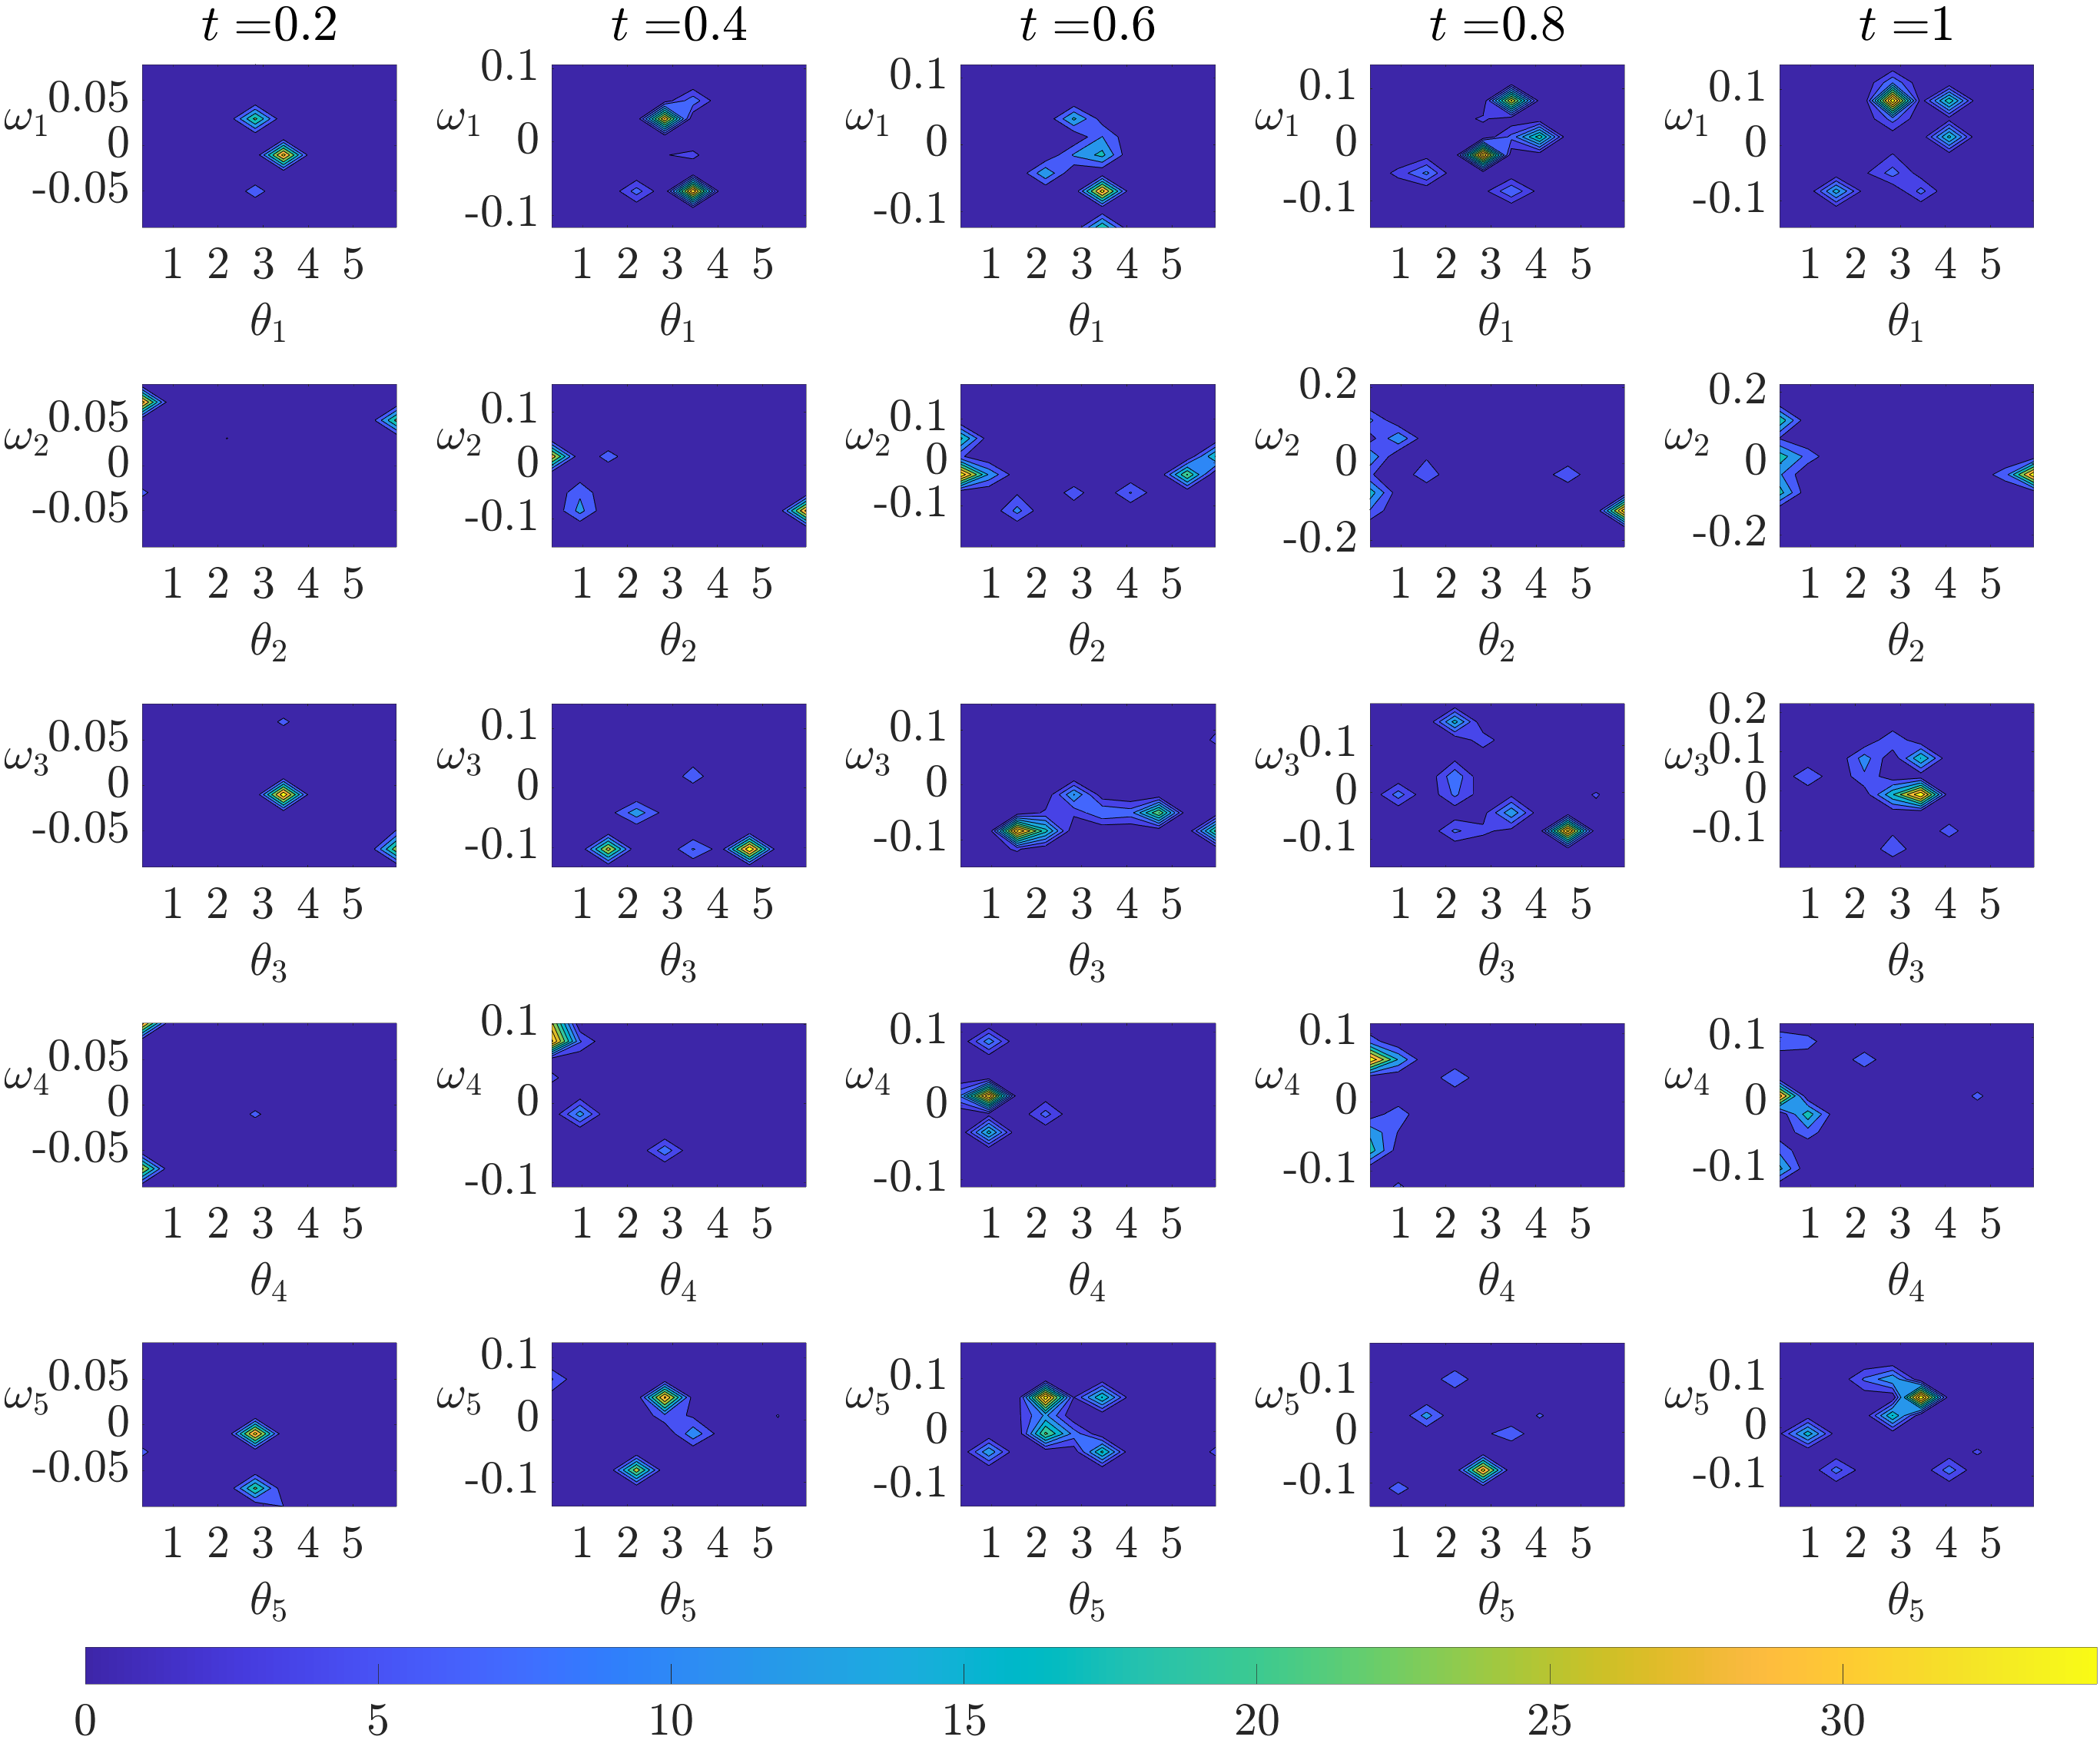
\includegraphics[width=0.99\linewidth]{IEEE14marginals.png}
\caption{\small{Example $(\theta_i,\omega_i)$ bivariate marginals, for the IEEE 14 bus system's generators $i=1,\hdots, 5$, shown as planar contour plots. The columns correspond to time snapshots; the rows correspond to the five generators. The colorbar corresponds to the value of the bivariate marginals. The simulation set up is described in Sec. V-A of the manuscript.}}
\vspace*{-0.1in}
\label{fig:PlanarContourBivariateMarginals}
\end{figure}



%%%%%%%%%%%%%%%%%%%%%%%%%%%%%%%%%%%%%%%%%%%%%%%%%%%%%%%%%%%%%%%%%%%%%%%%%%%%%%%%%%%%%%%%%%%%

\newpage
\section*{\large \bf Response to Reviewer \#4:}

\noindent
{\bf R4.1. Comments by reviewer}:\\
{\em The main contribution of this paper lies in applying results on the governing partial differential equation (PDE) for the joint PDF to avoid discretization of the state space, thereby circumventing computational challenges. The reviewer appreciates that this paper is rigorous in development and thinks it deals with an important problem.}

{\nib \blue{We appreciate the positive remark.}}


\noindent
{\bf R4.2. Comments by reviewer}:\\
{\em The key contribution of this paper is that the proposed method can reduce the computation burden when solving for the transient PDF. However, no comparison is provided with existing methods. The authors should provide comparisons to the exiting approaches, for example, based on finite element discretization or other numerical methods. The test example could be performed using the 5-generator system or larger systems. Besides, referring to Figs. 8 and 9, the total computation time should be reported for a longer horizon.}

{\nib \blue{ {\red{TBD.}}}}


\noindent
{\bf R4.3. Comments by reviewer}:\\
{\em Regarding the presentation, the reviewer suggests making the paper more self-contained. Some discussion in this paper highly relies on the authors' previous work, which can be improved by either adding a summarization or trimming out the materials.

Following the same vein, there are some unnecessary information and technical points provided in this paper that may be distracting.
For example, on page 3, why would the authors mention the Kuramoto oscillator model?
On page 4, is the detailed discussion regarding Wasserstein-2 metric necessary? Similarly, on page 5, the discussion about the natural energy functional and how the gradient drift case does not apply also seems too detailed.}

{\nib \blue{We have followed the reviewer's suggestion to improve the presentation. \ul{Specifically, in the revised manuscript's Sec. III-A, last two paragraphs summarize the technical relation of this paper w.r.t. the authors' previous work. In particular, we have added three more sentences with a new reference. To improve readability, have also broken what was a single paragraph in the previous version, into two separate paragraphs.} 

We appreciate the reviewer's point that the sentence containing equation (6) and the mention of Kuramoto model can be removed without affecting the rest of the development. However, we prefer to keep it since it adds didactic value, and many engineers may feel comfortable by the explicit mention that (1) is simply a rewriting of (6). Furthermore, an astute reader, encountering that sentence will realize that the scope of the technical contribution of this paper is broad because the algorithmic framework developed here will be applicable to several other non-power system applications (mentioned in the two cited references in that sentence) where the second order Kuramoto model is used. Since this is just a matter of one sentence, we will prefer to keep it. We hope you approve.

\ul{On the other hand, the detailed discussion regarding Wasserstein gradient flow and why that standard development cannot be applied in this case, is in fact, the heart of this paper}. \ul{A key contribution of this paper is to help distill out and tackle the core mathematical difficulty that hinders simply importing standard techniques from the optimal transport literature. To make the presentation tighter, in the revised manuscript, we have eschewed the Appendix and accordingly adjusted the material in Sec. III-D.}}}


\noindent
{\bf R4.4. Comments by reviewer}:\\
{\em Along with [25], there are recent developments that over-approximates the reachable set for nonlinear systems under uncertain initial conditions, parameters, and external disturbances:
``Reach-Set Estimation for DAE Systems under Uncertainty and Disturbances Using Trajectory Sensitivity and Logarithmic Norm".}

{\nib \blue{Thanks for providing that interesting recent reference. \ul{We have cited the same in the revised manuscript}.}}



\noindent
{\bf R4.5. Comments by reviewer}:\\
{\em On page 7, the authors stated about ``To account the pertinent geometry of $\mathbb{T}^n \times \mathbb{R}^n$". What exactly does this mean? Do the authors indicate that in (28) the two groups of state values are independent? Or do the authors mean the specific choices of the product von Mises PDF and the uniform distribution? If so, what are the connections?}

{\nib \blue{We simply mean that the joint PDF should be supported on $\mathbb{T}^n \times \mathbb{R}^n$, or a submanifold thereof. For instance, one cannot assume the initial joint PDF to be a $2n$ dimensional multivariate normal since that is supported over $\mathbb{R}^{2n}$, not over $\mathbb{T}^n \times \mathbb{R}^n$. It is, however, perfectly fine if some or all of the $2n$ components of the initial state vector are statistically correlated. As long as the support is $\mathbb{T}^n \times \mathbb{R}^n$, there is no issue if the angular variables are correlated with the Euclidean (i.e., angular velocity) variables.

}}


\noindent
{\bf R4.6. Comments by reviewer}:\\
{\em On page 5, is there a mistake in ``random samples from (28), and evaluated at (28)"?}

{\nib \blue{That was not a typo. Indeed, equation (28) was \ul{used in two ways}: it was used to generate initial state samples, and then the initial joint PDF values at those samples were evaluated via the functional form of (28), i.e., as in function evaluation. This is needed in our case because unlike standard Monte Carlo, we \ul{co-evolve} the state samples and joint PDF values at those state samples. \ul{To clarify this further, in the revised manuscript, we have slightly expanded that sentence}.}}


\noindent
{\bf R4.7. Comments by reviewer}:\\
{\em As a validation, it would be good to also provide information of higher-order moments along with the mean given in Fig. 10.}

{\nib \blue{ {\red{TBD.}}}}


\noindent
{\bf R4.8. Comments by reviewer}:\\
{\em There are some typos in this paper:\\
Page 4: in therms of\\
Page 5: in the right-hand side of the arrow in the expression following ``converges to the flow generated by (22)'', it should be plain $\rho$}

{\nib \blue{Corrected both. Thanks for pointing them out.}}




\end{document}
